
\chapter{Cadre g\'{e}ng\'{e}rale du projet}

\section{Introduction}

 Au cours de ce chapitre, nous  int\'{e}ressons par la
pr\'{e}sentation du contexte du travail ainsi que la pr\'{e}sentation de Start up
Cherchini pour laquelle ce travail a \'{e}t\'{e} r\'{e}alis\'{e}.
Puis nous passe par la th\'{e}matique du projet dans laquelle on va indiquer la
probl\'{e}matique, citer des produits existants sur le march\'{e}, sp\'{e}cifier les besoins
et indiquer la solution propos\'{e}e. Ainsi qu'on va d\'{e}crire la m\'{e}thodologie avec
laquelle on a pu concevoir et r\'{e}aliser notre projet, et on finit par la
pr\'{e}sentation de l'architecture de projet tout en en expliquant les choix
techniques et les outils n\'{e}cessaires.

\section{Contexte du travail}

 Ce stage s'inscrit dans le cadre d'un projet de fin d'\'{e}tudes pour l'obtention du
dipl\^{o}me Ing\'{e}nieur en informatique De l'Ecole Sup\'{e}rieure Priv\'{e}e des
Technologies de l'Information et de Management de Nabeul.

 Notre stage a \'{e}t\'{e} effectu\'{e} au sein de Start up Cherchini.
Le sujet est intitul\'{e} \guillemotleft{}Cr\'{e}ation d'une plateforme de gestion des projets\guillemotright{}




\section{Pr\'{e}sentation  de l'organisme d'accueil}

\bigskip
 Cherchini.tn est une agence de communication, cr\'{e}e en 2017, qui vous aide \`{a}
d\'{e}finir vos objectifs afin de vous fournir la solution web la plus adapt\'{e}e \`{a} vos
besoins. Cherchini.tn cherche souvent d'\^{e}tre \`{a} la pointe de l'innovation par sa
cr\'{e}ation graphique (logos, chartes graphiques, banni\`{e}res publicitaires,..),
cr\'{e}ation web, web design et r\'{e}f\'{e}rencement des sites web.

\bigskip
 En outre, Cherchini.tn vous offre des solutions de vente en ligne, son objectif
est de mettre en relation les clients et les vendeurs dans le but de r\'{e}aliser de
tr\`{e}s bonnes affaires tout en b\'{e}n\'{e}ficiant de ses expertises.

Site Web : https://cherchini.tn/

\bigskip

  \FloatBarrier
\begin{figure}[H]
\center

\includegraphics[width=10cm,height=9cm]{./figures/cherchini-logo.png}
\caption{Logo de Cherchini.}

\end{figure}


\section{Contexte du projet }
Ce stage s'inscrit dans le cadre d'un projet de fin d'\'{e}tudes pour l'obtention du
dipl\^{o}me Ing\'{e}nieur en informatique De l'Ecole Sup\'{e}rieure Priv\'{e}e des
Technologies de l'Information et de Management de Nabeul.
Notre stage a \'{e}t\'{e} effectu\'{e} au sein de Start up Cherchini.
Le sujet est intitul\'{e} \guillemotleft{}Cr\'{e}ation d'une plateforme de gestion des projets\guillemotright{}


%\subsection{Business intelligence}
% L'informatique d\'{e}cisionnelle, aussi appel\'{e}e business intelligence(BI), d\'{e}signe un ensemble de m\'{e}thodes, de moyens et d'outils %informatiques utilis\'{e}s pour piloter une entreprise et aider \`{a} la prise de d\'{e}cision : tableaux de bord, rapports analytiques et prospectifs.

\section{ Etude de l'existant  }



Il existes sur le march\'{e} plusieurs plateformes de gestion des projet , et parmi
les outils les plus connues on trouve ASANA et JIRA .

\subsection{Asana}

Il s'agit d'une plate-forme robuste qui sert \`{a} vos \'{e}quipes de rester concentr\'{e}es
sur les objectifs, les projets et les t\^{a}ches quotidiennes .Voici les
fonctionnalit\'{e}s les plus importantes qu'elle offre :


\begin{itemize}
\item{Tableau de bord permet de visualiser facilement votre travail.}

\item{ Voir la grande image. Clouez votre timing en visualisant les travaux sur
un calendrier. Rep\'{e}rez facilement les trous et les chevauchements dans
votre horaire et effectuez rapidement les ajustements n\'{e}cessaires.}

\item{Gardez une trace de ce qui est le plus important.}

\item{Pas besoin de r\'{e}inventer la roue. Transformez les processus courants en
mod\`{e}les que votre \'{e}quipe enti\`{e}re peut utiliser pour que les projets se
d\'{e}roulent sans heurts \`{a} chaque fois.}

\item{Partagez des informations avec les bonnes personnes. Rendez les
\'{e}quipes et les projets priv\'{e}s afin de cr\'{e}er un espace s\'{e}curis\'{e} pour les
travaux sensibles.}

\item{Partagez des informations avec les bonnes personnes. Rendez les
\'{e}quipes et les projets priv\'{e}s afin de cr\'{e}er un espace s\'{e}curis\'{e} pour les
travaux sensibles.}

\end{itemize}

\subsection{Jira}
Qui est l'un des meilleurs outils de gestion de produit qui comprend :
\begin{itemize}

\item{Le suivi et la gestion des probl\`{e}mes}

\item{La gestion des produits}

\item{Un Tableau de bord configurable}

\item{Des Rapport sur l'avancement du projet}

\item{Support des m\'{e}thodologies Scrum \& Kanban}

\end{itemize}



\section{ Probl\'{e}matique }
Toute entreprise aspire \`{a} se conformer au triangle d'or (D\'{e}lai, Cout, Qualit\'{e})
autour du quel tournent tous les projets professionnelles.(Figure 1.2)




Dans le but d'organiser ses projets, Cherchini veut r\'{e}aliser son propre outil de
gestion des projets, en fait, l'absence d'un tel outil demeurent inaper\c{c}ue
pour les premi\`{e}res ann\'{e}es d'une nouvelle entreprise et surtout pour les
petites ou moyenne entreprises, mais \'{e}videmment, cela va engendrer au futur
une mal organisation et une perte des informations importantes, et en
cons\'{e}quence une perte de temps et d'argent.

On remarque alors que les outils existants sont assez sophistiqu\'{e}s.
Ainsi que ces deux outils, ils existent plusieurs concurrents qui offrent
plusieurs manipulations et possibilit\'{e}s.
Les fonctionnalit\'{e}s sont payantes pour chacun de ces outils et Cherchini n'a
pas besoin de tous ces fonctionnalit\'{e}s d'une part, et d'autre part elle voudrait
\^{e}tre capable d'\'{e}tendre certaines fonctionnalit\'{e}s et de les r\'{e}duire selon le
besoin .Par exemple, ajouter une carte g\'{e}ographique qui indique la
g\'{e}olocalisation de ses partenaires dans cette plateforme .
Pour cela, Cherchini voudrais avoir son propre outil de gestion de projet et d\'{e}sire r\'{e}aliser un
service d'informatique d\'{e}cisionnelle (Business Intelligence) ,ce service doit donner une vue g\'{e}n\'{e}rale sur le d\'{e}roulement des projets
selon les couts et les d\'{e}lais \`{a} suivre.


\begin{figure}[H]
\center
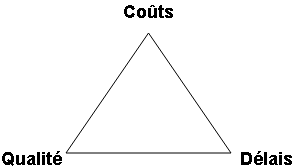
\includegraphics[width=8cm,height=5cm]{./figures/triangle.png}
\caption{Triangle d'or.}
\end{figure}




\section{ Solution propos\'{e}e  }
Pour r\'{e}pondre aux besoins fonctionnels, nous avons construit une application web en
se basant sur l’architecture suivante.


\begin{figure}
\center
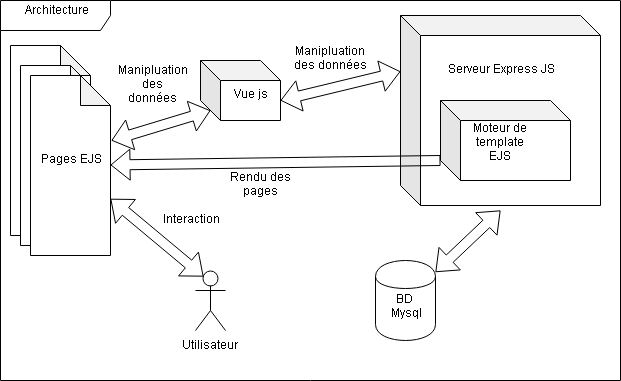
\includegraphics[width=10cm,height=10cm]{./figures/archi.png}
\caption{Architecture g\'{e}n\'{e}rale.}
\end{figure}

Comme nous avons indiqu\'{e}, pour \^{e}tre capable d'\'{e}tendre les fonctionnalit\'{e}s
selon le besoin en \'{e}vitant la complexit\'{e} des outils existantes et les couts de
paiement pour chaque fonctionnalit\'{e}, on a adopt\'{e} des technologies open
sources et gratuits, et voici les technologies qu'on a utilis\'{e}:

\begin{itemize}

\item{Pour la base de donn\'{e}es : MYSQL}
\item{Pour le serveur et API REST : Express JS ,NODE JS}
\item{Moteur de Template (engine view) : EJS(Embedded JavaScript) }
\item{Pour les pages web : HTML(HyperText Markup Language,) et Vue js}
\item{Pour l'authentification : JWT(JSON Web Token) }
\item{Pour la carte de g\'{e}olocalisation des clients : LeafLet maps}
\item{Pour le diagramme de Gantt et les rapport : Highcharts}

\end{itemize}

\section{ Etude m\'{e}thodologique }



  \subsection{Choix de la   m\'{e}thodologie}

  Dans la plupart des projets, on a besoin de suivre un processus qui d\'{e}finit
QUI fait QUOI, QUAND et COMMENT pour \^{e}tre capable de :

\begin{itemize}
\item{Atteindre un certain objectif.}
\item{Construire des mod\`{e}les d'un ou de plusieurs syst\`{e}mes.}
\item{G\'{e}rer le cycle de vie du projet de A \`{a} Z.}
\item{Organiser le projet}
\item{G\'{e}rer les risques}
\item{Obtenir de mani\`{e}re r\'{e}p\'{e}titive des produits de qualit\'{e} constante}
\end{itemize}

Le choix entre une m\'{e}thode et une autre, d\'{e}pend de la nature du projet et de sa taille. Pour des
projets de petite taille et dont le domaine est ma\^{\i}tris\'{e}, par exemple, un cycle de vie en cascade
s'av\`{e}re largement su Sant. Lorsqu'il s'agit d'un projet o\`{u} les donn\'{e}es ne sont pas r\'{e}unies d\`{e}s le
d\'{e}part, o\`{u} les besoins sont incomplets voire floues, il faut s'orienter vers une m\'{e}thode it\'{e}rative
ou orient\'{e}es prototypes.
Parmi les m\'{e}thodes it\'{e}ratives, nous pouvons distinguer les m\'{e}thodes agiles largement utilis\'{e}es
de nos jours \`{a} travers le monde. Une m\'{e}thode agile est men\'{e}e dans un esprit collaboratif et
s'adapte aux approches incr\'{e}mentales. Elle engendre des produits de haute qualit\'{e} tout en tenant
compte de l'\'{e}volution des besoins du client.
La nature de projet qui doit \^{e}tre \'{e}volutif et dont tous les besoins n'ont pas encore \'{e}t\'{e}
totalement identit\'{e}s, nous a orient\'{e}es vers une m\'{e}thode de type agile et plus particuli\`{e}rement
SCRUM.
  \subsection{Pr\'{e}sentation de la m\'{e}thodologie SCRUM}
Scrum signifie m\^{e}l\'{e}e au rugby. Il exploite les valeurs et l'esprit du rugby et les adapte aux
projets de d\'{e}veloppement. Comme le pack lors d'un ballon port\'{e} au rugby, l'\'{e}quipe charg\'{e}e du
d\'{e}veloppement de travaille de fa\c{c}on collective, soud\'{e}e vers un objectif pr\'{e}cis. Comme un demi
de m\^{e}l\'{e}e, le ScrumMaster est le responsable du projet qui oriente les membres de l'\'{e}quipe dans
la bonne direction, assure l'environnement de travail et chercher \`{a} am\'{e}liorer la productivit\'{e} et
le savoir faire de don \'{e}quipe.
Scrum se base sur la th\'{e}orie du contr\^{o}le empirique de processus. L'empirisme mentionne que
les connaissances proviennent de l'exp\'{e}rience et d'une prise de d\'{e}cision bas\'{e}e sur des faits
connus. Scrum utilise une approche it\'{e}rative et incr\'{e}mentale pour optimiser la pr\'{e}dictibilit\'{e} et
contr\^{o}ler le risque.
\begin{figure}[H]
\center
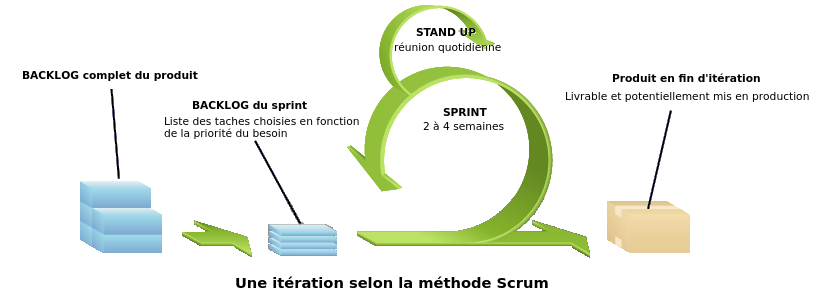
\includegraphics[width=10cm,height=6cm]{./figures/scrum.png}
\caption{M\'{e}thodologie scrum.}

\end{figure}

Comme nous pouvons le remarquer dans cette figure, pour mettre en place la m\'{e}thode
SCRUM, il faut tout d'abord d\'{e}finir les diff\'{e}rentes fonctionnalit\'{e}s de notre application qui
forment le Backlog du produit. Ensuite, nous proc\'{e}dons \`{a} la planification du sprint pour d\'{e}finir
le plan d\'{e}taill\'{e} d'une it\'{e}ration. Les sprints durent g\'{e}n\'{e}ralement deux \`{a} quatre semaines. Durant
un sprint, il y a toujours des r\'{e}unions quotidiennes entre les diff\'{e}rents collaborateurs du projet
pour pr\'{e}senter l'\'{e}tat d'avancement des diff\'{e}rentes t\^{a}ches en cours, les difficult\'{e}s rencontr\'{e}es
ainsi que les t\^{a}ches restantes \`{a} r\'{e}aliser. Une fois le produit partiel est pr\^{e}t, nous v\'{e}rifions la
conformit\'{e} de ce qui a \'{e}t\'{e} fait durant le sprint et nous pouvons alors l'am\'{e}liorer en proc\'{e}dant \`{a}
l'\'{e}tape de r\'{e}trospective.


\subsection{Planning du projet}
Le tableau suivant résume les \'{e}tapes que nous avons suivies:


\begin{table}

\begin{tabular}{|l|l|l|}
\hline
Backlog                         & Sprint                                                                                                                                         & Durée                 \\
\hline
\multirow{5}{*}{Etape Initiale} & Recherche sur les nouvelles technologies qu’on va utiliser                                                                                     & 3 Semaines            \\
\cline{2-3}
                                & Formation sur les langages                                                                                                                     & 3 Semaines            \\
\cline{2-3}
                                & Rédaction du chapitre présentation de cadre générale                                                                                           & 2 jours               \\
\cline{2-3}
                                & \begin{tabular}[c]{@{}l@{}}Création des diagrammes (Diagramme de classe, \\Diagramme de séquence, Diagramme de cas d’utilisation)\end{tabular} & 3 Semaines            \\
\cline{2-3}
                                & Rédaction du chapitre spécification des besoins                                                                                                & 2 jours               \\
\hline
\multicolumn{3}{|l|}{Réunion}                                                                                                                                                                            \\
\hline
\multirow{5}{*}{Etape 2}        & \begin{tabular}[c]{@{}l@{}}Création des premières interfaces de l’application(Gestion\\~des membres \\,clients ,projet ,tâches ) \end{tabular} & 1 Semaine             \\
\cline{2-3}
                                & Rédaction du chapitre conception                                                                                                               & 2 jours               \\
\cline{2-3}
                                & Création diagramme de Gantt                                                                                                                    & 1 jour                \\
\cline{2-3}
                                & Maintenance et test de la fonctionnalité gestion de projet                                                                                     & 2 jours               \\
\cline{2-3}
                                & Développement de l’interface Gannt et de la carte géographique                                                                                 & 2 jours               \\
\hline
\multicolumn{3}{|l|}{Réunion}                                                                                                                                                                            \\
\hline
\multirow{2}{*}{Etape 3}        & Développement de~L’interface membre                                                                                                            & 1 Semaine             \\
\cline{2-3}
                                & Développement de la partie Authentification                                                                                                    & 1 Semaine             \\
\hline
\multicolumn{3}{|l|}{Réunion}                                                                                                                                                                            \\
\hline
\multirow{2}{*}{Etape 4}        & Développement de la partie~ETL                                                                                                                 & 3 jours               \\
\cline{2-3}
                                & Ajouter les rapports à l’interface administrateur                                                                                              & 1 jour                \\
\hline
\multicolumn{3}{|l|}{Réunion}                                                                                                                                                                            \\
\hline
\multirow{2}{*}{Etape finale}   & Dernières retouches sur le design de~l’application                                                                                             & 3 jours               \\
\cline{2-3}
                                & Mises à jour du~rapport                                                                                                                        & 3 jours               \\
\hline
\multicolumn{1}{l}{}            & \multicolumn{1}{l}{}                                                                                                                           & \multicolumn{1}{l}{}  \\
\multicolumn{1}{l}{}            & \multicolumn{1}{l}{}                                                                                                                           & \multicolumn{1}{l}{}  \\
\multicolumn{1}{l}{}            & \multicolumn{1}{l}{}                                                                                                                           & \multicolumn{1}{l}{}
\end{tabular}
\centering
\caption{ Planning du projet}
\end{table}


\subsection{Diagramme de Gantt}


\begin{figure}[H]

\begin{center}
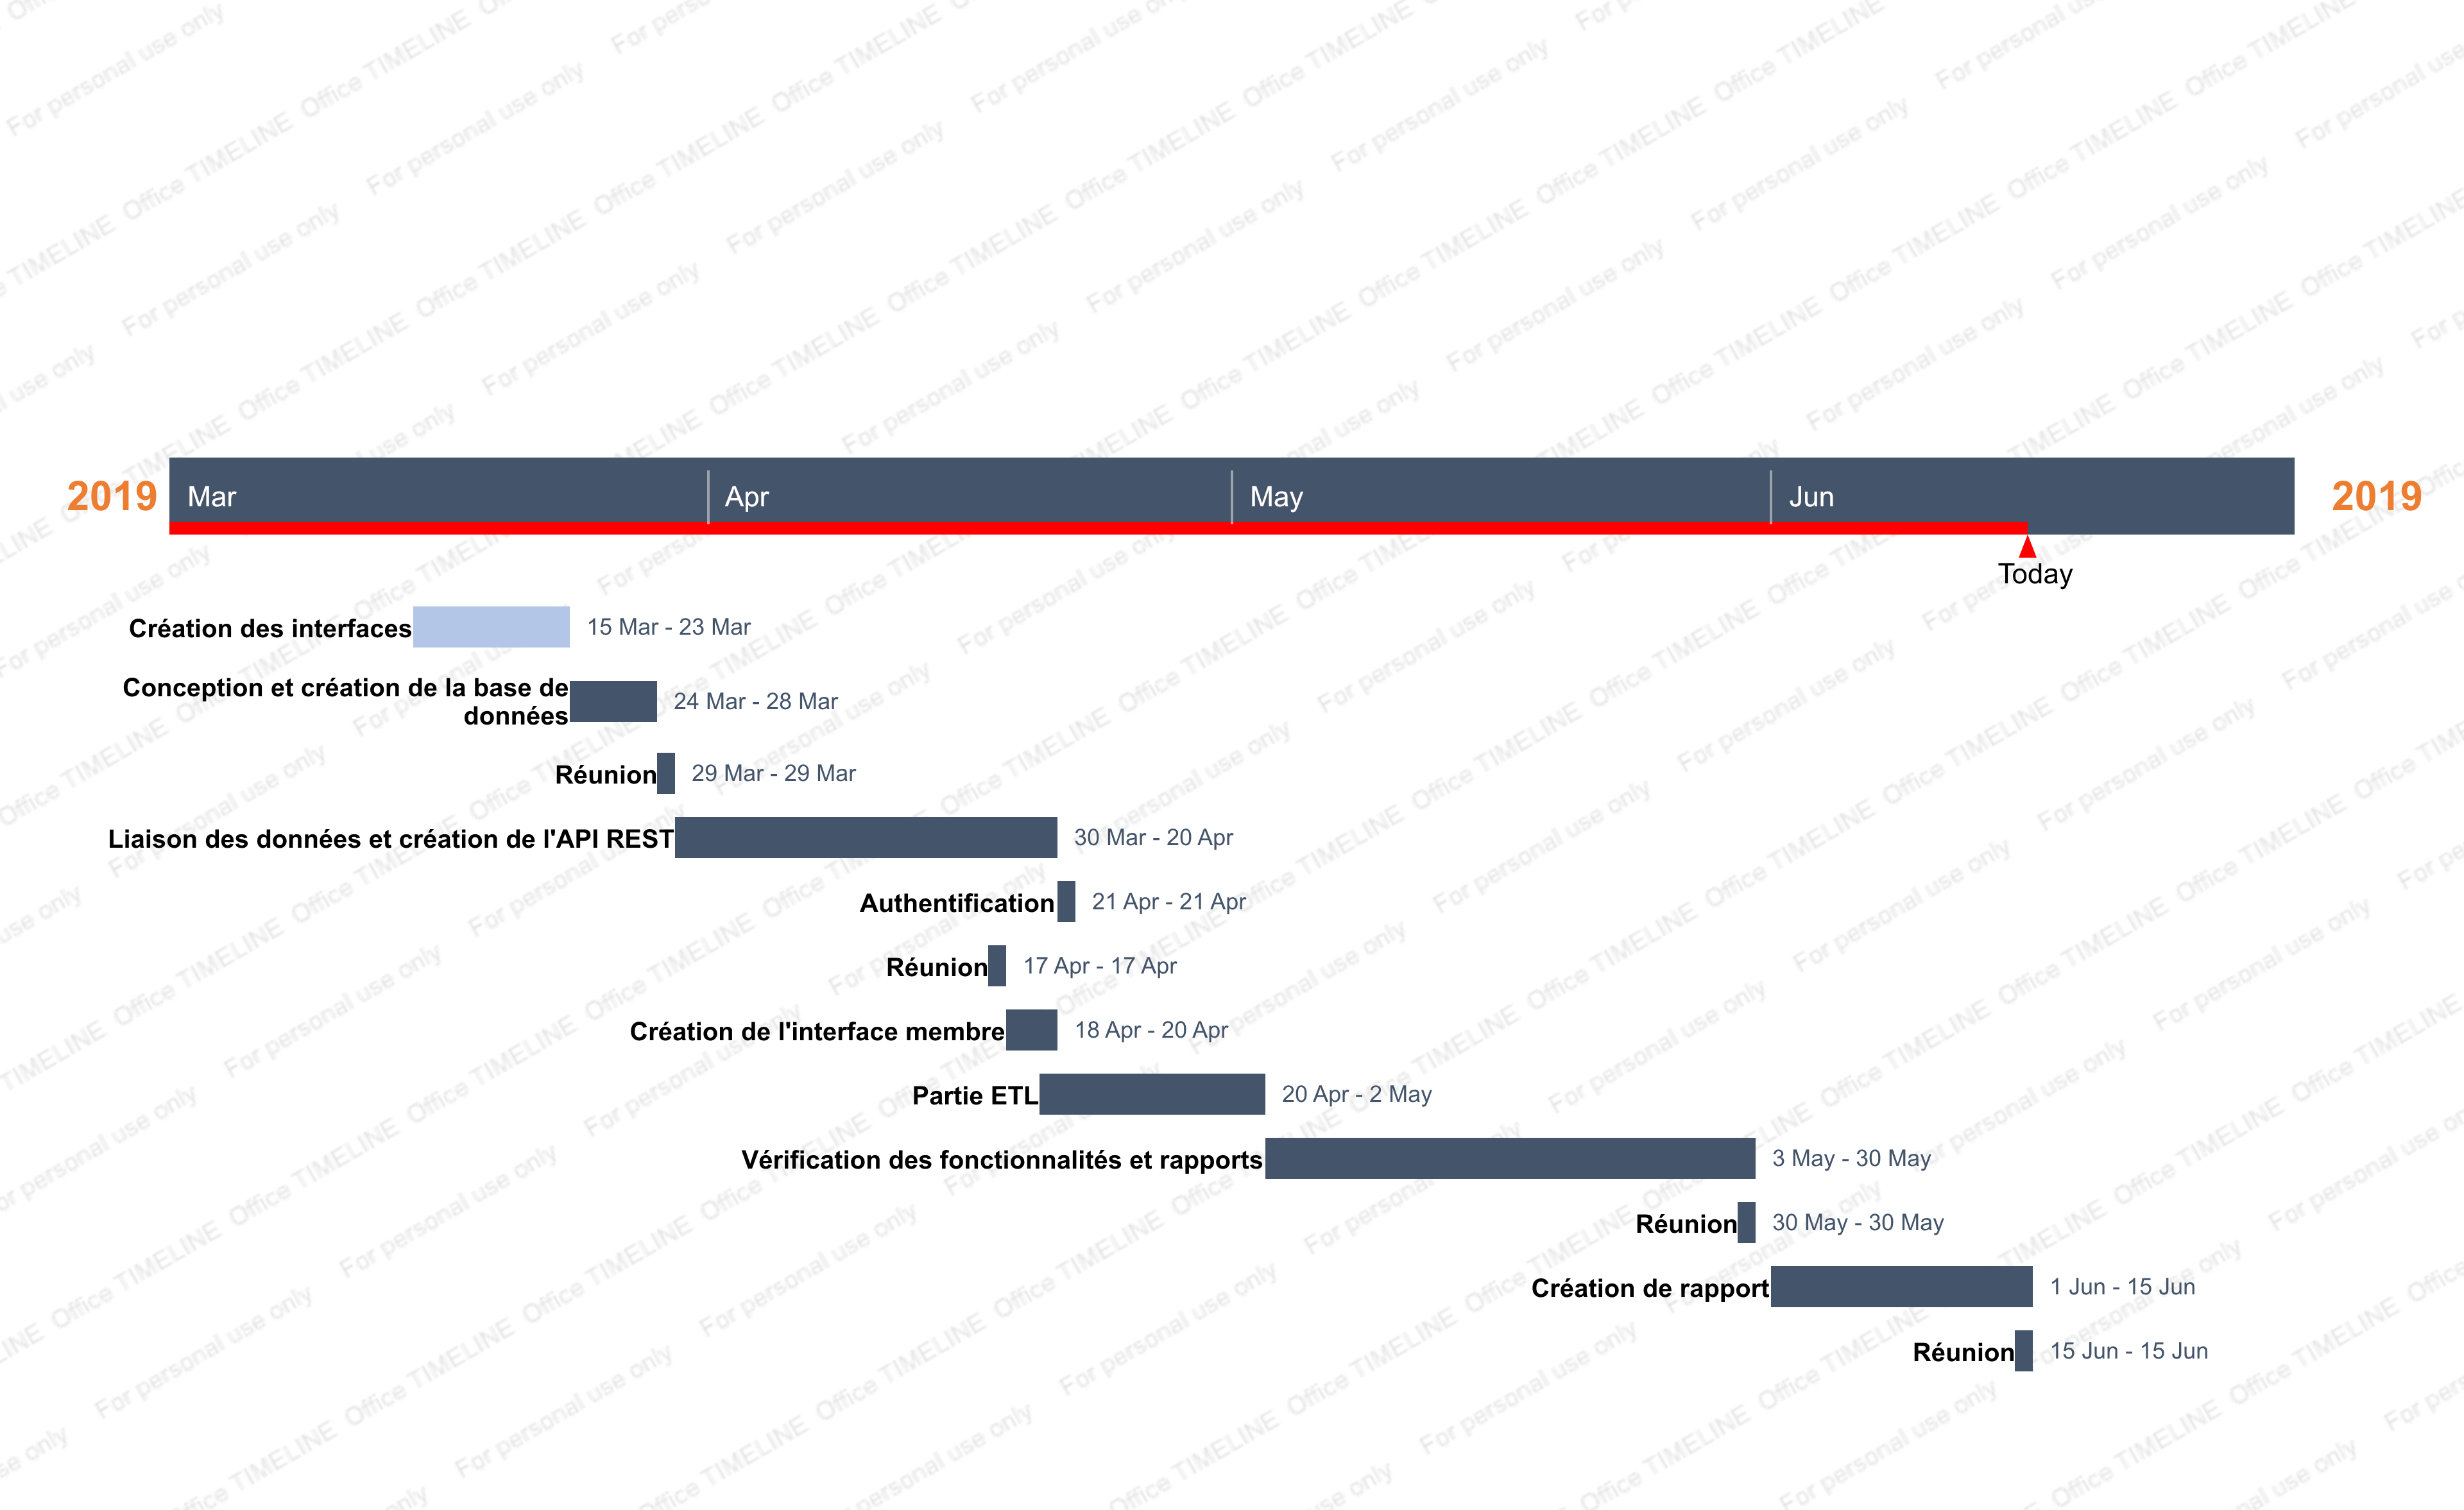
\includegraphics[width=17cm,height=15cm]{./figures/gantt.png}
\caption{Diagramme de Gantt.}
\end{center}
\end {figure}
